% !TEX root = ../main.tex
% File: chapters_part1/chap4_2.tex
% Nội dung cho Chương 4, Phần 2

\section{Phân loại Kiến trúc LLMs}
\label{sec:llm_architectures_classification}

Kiến trúc Transformer gốc mà chúng ta vừa phân tích là một mô hình Encoder-Decoder hoàn chỉnh, được thiết kế cho các tác vụ chuỗi-sang-chuỗi (sequence-to-sequence). Tuy nhiên, các nhà nghiên cứu nhanh chóng nhận ra rằng bằng cách chỉ sử dụng một phần của kiến trúc này -- hoặc chỉ Encoder, hoặc chỉ Decoder -- họ có thể tạo ra các mô hình được chuyên môn hóa cao và cực kỳ hiệu quả cho các loại tác vụ khác nhau.

Sự phân tách này đã khai sinh ra ba "họ" kiến trúc chính, định hình nên toàn bộ bối cảnh của các Mô hình Ngôn ngữ Lớn (LLMs) ngày nay. Hiểu rõ ba họ kiến trúc này là chìa khóa để lựa chọn mô hình phù hợp cho ứng dụng của bạn.

\subsection{Họ Mô hình chỉ Encoder (Encoder-Only): Bậc thầy của Sự Hiểu Ngôn ngữ}
\label{ssec:encoder_only}

Các mô hình thuộc họ này chỉ sử dụng khối Encoder của kiến trúc Transformer. Chúng được thiết kế với một mục tiêu duy nhất: tạo ra các \textbf{biểu diễn ngữ cảnh sâu sắc (deep contextualized representations)} cho văn bản đầu vào.

\begin{tcolorbox}[
    title=Triết lý của Encoder-Only,
    colback=blue!5!white, colframe=blue!75!black, fonttitle=\bfseries
]
"Để thực sự hiểu ý nghĩa của một từ trong câu, tôi cần phải nhìn vào \textbf{cả hai phía}: những từ đứng trước nó và những từ đứng sau nó."
\end{tcolorbox}

\subsubsection{Kiến trúc và Mục tiêu Huấn luyện Nền tảng}
\paragraph{Kiến trúc và Tính hai chiều (Bidirectionality)}
Đây là đặc điểm quan trọng nhất. Nhờ cơ chế Self-Attention không bị che (unmasked), tại mỗi lớp, mỗi từ có thể "chú ý" đến tất cả các từ khác trong câu, cả bên trái và bên phải. Điều này cho phép mô hình xây dựng một sự hiểu biết toàn diện về ngữ cảnh, điều mà các mô hình hồi tiếp (RNN) hay tự hồi quy (Decoder-Only) không thể làm được. Đầu ra của mô hình là một chuỗi các vector embedding, mỗi vector tương ứng với một token đầu vào, nhưng đã được "làm giàu" bởi thông tin ngữ cảnh hai chiều sâu sắc.

\paragraph{Mục tiêu Huấn luyện: Masked Language Modeling (MLM)}
MLM là mục tiêu huấn luyện cốt lõi của BERT và nhiều mô hình kế nhiệm.
\begin{itemize}
    \item \textbf{Cơ chế:} Lấy một câu đầu vào, che (mask) ngẫu nhiên khoảng 15\% số token bằng một token đặc biệt `[MASK]`. Sau đó, nhiệm vụ của mô hình là \textbf{dự đoán các token gốc đã bị che}, dựa vào các token không bị che xung quanh.
    \item \textbf{Tại sao lại hiệu quả?} MLM buộc mô hình phải học các mối quan hệ ngữ nghĩa và cú pháp sâu sắc từ cả hai phía để có thể "điền vào chỗ trống". Nó không chỉ là dự đoán từ tiếp theo, mà là một bài kiểm tra "đọc hiểu" thực sự.
\end{itemize}

\begin{center}
    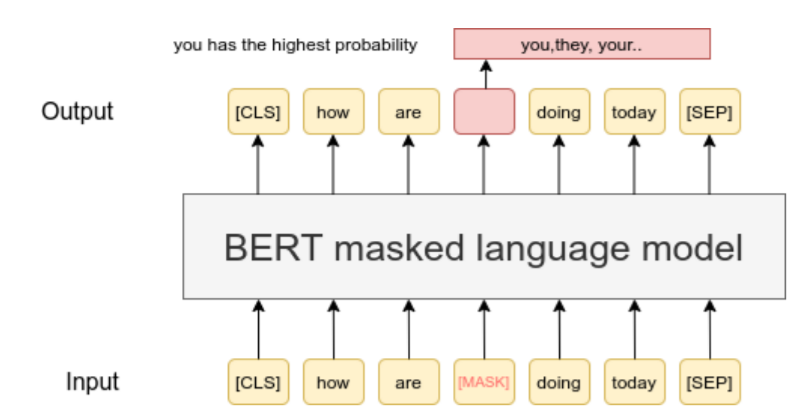
\includegraphics[width=0.8\textwidth]{bert_mlm_nsp.png}
    \captionof{figure}{Mục tiêu huấn luyện kinh điển của BERT: Masked Language Modeling (MLM). Mô hình phải dự đoán các token bị che dựa trên ngữ cảnh hai chiều.}
    \label{fig:bert_mlm_nsp}
\end{center}

\subsubsection{Sự phát triển và các biến thể của Họ Encoder-Only}
Từ nền tảng của BERT, một hệ sinh thái đa dạng các mô hình Encoder-Only đã ra đời, mỗi loại được tối ưu cho các mục đích khác nhau: hiệu suất, kích thước, tác vụ cụ thể, hay miền kiến thức chuyên biệt.

\paragraph{1. Gia đình BERT: Những người kế nhiệm trực tiếp}
Đây là các mô hình cải tiến trực tiếp từ kiến trúc và phương pháp huấn luyện của BERT.
\begin{itemize}
    \item \textbf{RoBERTa (Facebook) \cite{liu2019roberta}:} Không thay đổi kiến trúc, nhưng chứng minh rằng việc tối ưu hóa kỹ lưỡng quá trình huấn luyện có thể mang lại hiệu quả vượt trội. Các cải tiến chính bao gồm: huấn luyện lâu hơn, trên nhiều dữ liệu hơn, với batch size lớn hơn, loại bỏ mục tiêu NSP (Next Sentence Prediction), và sử dụng "che động" (dynamic masking).
    \item \textbf{DistilBERT (Hugging Face) \cite{sanh2019distilbert}:} Một phiên bản "chưng cất" nhỏ hơn, nhanh hơn của BERT. Nó sử dụng kỹ thuật \textit{knowledge distillation}, trong đó một mô hình "học trò" (student) nhỏ hơn học cách bắt chước đầu ra của một mô hình "giáo viên" (teacher) lớn hơn (BERT). DistilBERT giữ lại 97\% hiệu năng của BERT nhưng chỉ có 60\% kích thước.
    \item \textbf{ALBERT (Google) \cite{lan2019albert}:} Một cách tiếp cận khác để giảm tham số. ALBERT sử dụng hai kỹ thuật chính: \textit{factorized embedding parameterization} (phân tách ma trận embedding từ lớn thành hai ma trận nhỏ) và \textit{cross-layer parameter sharing} (chia sẻ trọng số của các khối Transformer với nhau).
    \item \textbf{SpanBERT (Facebook) \cite{joshi2020spanbert}:} Tối ưu hóa BERT cho các tác vụ cần hiểu các \textbf{đoạn văn bản (spans)} liên tục, như Hỏi-đáp trích xuất. Thay vì che các token ngẫu nhiên, SpanBERT che các đoạn ngẫu nhiên và huấn luyện mô hình dự đoán toàn bộ đoạn bị che chỉ từ các token ở biên của đoạn đó.
\end{itemize}

\paragraph{2. Các mô hình Biểu diễn Câu: Chuyên gia về Tìm kiếm Ngữ nghĩa}
Một hạn chế của BERT gốc là nó không tạo ra các vector biểu diễn câu (sentence embeddings) tốt "ngay lập tức". Việc lấy embedding của token `[CLS]` hoặc lấy trung bình các token embedding thường cho kết quả tìm kiếm tương đồng không cao. Nhánh mô hình này giải quyết vấn đề đó.
\begin{itemize}
    \item \textbf{SBERT (Sentence-BERT) \cite{reimers2019sentence}:} Là mô hình tiên phong. SBERT tinh chỉnh BERT trên các cặp câu bằng cách sử dụng kiến trúc \textit{siamese} hoặc \textit{triplet}. Kiến trúc này buộc mô hình phải tạo ra một không gian vector mà ở đó các câu có ngữ nghĩa giống nhau sẽ có vector gần nhau (cosine similarity cao) và ngược lại.
    \item \textbf{SimCSE (Simple Contrastive Sentence Embedding) \cite{gao2021simcse}:} Một phương pháp học tương phản (contrastive learning) đơn giản nhưng cực kỳ hiệu quả. Để tạo một cặp dương, SimCSE chỉ cần đưa cùng một câu qua mô hình BERT hai lần (với dropout khác nhau). Các câu khác trong batch được coi là cặp âm. Kỹ thuật này tạo ra các embedding câu chất lượng rất cao mà không cần dữ liệu gán nhãn.
    \item \textbf{E5 (Embeddings from bidErectional Encoder rEpresentations \cite{wang2022text}), Contriever, etc.:} Là thế hệ mô hình embedding mới nhất, được huấn luyện đặc biệt cho các tác vụ \textbf{tìm kiếm (retrieval)}, đặc biệt là tìm kiếm bất đối xứng (truy vấn ngắn, tài liệu dài). Chúng thường đạt hiệu năng SOTA trên các benchmark tìm kiếm ngữ nghĩa.
\end{itemize}

\paragraph{3. Các mô hình cho Miền chuyên biệt và Đa ngôn ngữ}
Ý tưởng cốt lõi là một mô hình được huấn luyện trước trên dữ liệu chuyên ngành sẽ hiểu thuật ngữ và ngữ cảnh của ngành đó tốt hơn.
\begin{itemize}
    \item \textbf{SciBERT \cite{beltagy2019scibert}, BioBERT \cite{lee2020biobert}, ClinicalBERT \cite{alsentzer2019publicly}:} Được huấn luyện trên các kho văn bản khoa học, y sinh, và y tế lâm sàng.
    \item \textbf{FinBERT:} Chuyên cho lĩnh vực tài chính.
    \item \textbf{LegalBERT:} Chuyên cho lĩnh vực pháp luật.
    \item \textbf{CamemBERT \cite{martin2019camembert} (Pháp), PhoBERT \cite{nguyen2020phobert} (Việt), etc.:} Là các mô hình theo kiến trúc RoBERTa nhưng được huấn luyện từ đầu trên kho dữ liệu lớn của một ngôn ngữ cụ thể, cho hiệu năng vượt trội so với các mô hình đa ngôn ngữ trên ngôn ngữ đó.
\end{itemize}

\paragraph{4. Các Encoder Hiện đại, Gọn nhẹ và Hiệu quả}
Nhánh này tập trung vào việc tạo ra các mô hình nhỏ gọn hơn nhưng vẫn giữ được hiệu năng cao thông qua các cải tiến về kiến trúc và mục tiêu huấn luyện.
\begin{itemize}
    \item \textbf{MiniLM (Microsoft) \cite{wang2020minilm}:} Sử dụng một phương pháp chưng cất tri thức sâu, trong đó mô hình học trò không chỉ bắt chước đầu ra cuối cùng mà còn cả ma trận chú ý và mối quan hệ giữa các vector value từ mô hình giáo viên.
    \item \textbf{DeBERTa (Microsoft) \cite{he2020deberta}:} Một trong những encoder mạnh nhất hiện nay. DeBERTa giới thiệu cơ chế \textit{disentangled attention}, tách rời việc mã hóa nội dung từ và vị trí tương đối của chúng.
    \item \textbf{MPNet (Microsoft) \cite{song2020mpnet}:} Kết hợp τα tốt nhất của cả hai thế giới: MLM (BERT) và Permuted Language Modeling (XLNet). Nó giải quyết sự không tương thích giữa pre-training và fine-tuning, cho phép mô hình học các phụ thuộc hai chiều một cách toàn diện hơn.
\end{itemize}

\paragraph{5. Các Encoder với Mục tiêu Huấn luyện khác MLM}
MLM không phải là cách duy nhất để huấn luyện một encoder hai chiều.
\begin{itemize}
    \item \textbf{ELECTRA (Google) \cite{clark2020electra}:} Sử dụng một tác vụ hiệu quả hơn là \textit{replaced token detection}. Một mô hình "generator" nhỏ sẽ thay thế một số token trong câu, và mô hình "discriminator" (chính là ELECTRA) phải dự đoán xem mỗi token là gốc hay đã bị thay thế. Tác vụ này hiệu quả hơn vì mô hình học từ \textit{tất cả} các token, không chỉ 15% bị che.
    \item \textbf{XLNet (Google/CMU) \cite{yang2019xlnet}:} Một mô hình \textit{tự hồi quy hoán vị (permutation-based autoregressive)}. Nó dự đoán các token trong câu theo một thứ tự ngẫu nhiên. Bằng cách này, nó có thể "nhìn thấy" ngữ cảnh từ cả hai phía (giống BERT) trong khi vẫn giữ được các lợi ích của mô hình tự hồi quy.
\end{itemize}

\begin{tcolorbox}[
    title=Tổng kết: Điểm mạnh và Ứng dụng của Encoder-Only,
    colback=blue!5!white, colframe=blue!75!black, fonttitle=\bfseries
]
\textbf{Nguyên tắc chung:} Sử dụng mô hình Encoder-Only khi tác vụ của bạn đòi hỏi sự \textbf{hiểu sâu sắc về toàn bộ văn bản đầu vào} và đầu ra không phải là một chuỗi văn bản mới, mạch lạc. Chúng là các mô hình \textbf{NLU (Natural Language Understanding)} chứ không phải \textbf{NLG (Natural Language Generation)}.

\textbf{Ứng dụng điển hình:}
\begin{itemize}
    \item \textbf{Phân loại văn bản (Text Classification):} Phân tích cảm xúc, phát hiện chủ đề, kiểm duyệt nội dung (toxic detection). Mô hình cần hiểu toàn bộ câu để đưa ra một nhãn duy nhất.
    \item \textbf{Gán nhãn chuỗi (Token Classification):} Nhận dạng Thực thể Tên (NER), Gán nhãn Từ loại (POS Tagging). Mô hình cần hiểu ngữ cảnh xung quanh mỗi từ để gán nhãn cho nó.
    \item \textbf{Tìm kiếm Ngữ nghĩa (Semantic Search):} Biến các câu/tài liệu thành các vector embedding có ý nghĩa (sử dụng các mô hình như SBERT, E5). Các vector này sau đó được lưu trữ và truy vấn bằng các thuật toán tìm kiếm lân cận gần nhất (ANN).
    \item \textbf{Hỏi-đáp trích xuất (Extractive QA):} Tìm và trích xuất một đoạn văn bản (span) làm câu trả lời từ một văn bản ngữ cảnh cho trước.
    \item \textbf{Retrieval-Augmented Generation (RAG):} Đây là một ứng dụng lai. Giai đoạn \textbf{Retrieval (Truy xuất)} trong RAG sử dụng một mô hình Encoder-Only (như E5) để biến truy vấn của người dùng và các tài liệu trong cơ sở tri thức thành vector, sau đó tìm ra các tài liệu liên quan nhất. Các tài liệu này sau đó mới được đưa cho một mô hình sinh (Decoder-Only) để tạo ra câu trả lời.
\end{itemize}
\end{tcolorbox}

\subsection{Họ Mô hình chỉ Decoder (Decoder-Only): Bậc thầy của Sự Sáng tạo}
\label{ssec:decoder_only}
Đây là họ kiến trúc đang thống trị thế giới AI hiện nay, là nền tảng của các mô hình như ChatGPT, Llama, và Claude. Chúng chỉ sử dụng khối Decoder của kiến trúc Transformer.

\begin{tcolorbox}[
    title=Triết lý của Decoder-Only,
    colback=red!5!white, colframe=red!75!black, fonttitle=\bfseries
]
"Để viết tiếp một câu chuyện, tôi chỉ cần biết những gì đã được viết \textbf{trước đó}. Tôi không được phép nhìn vào tương lai."
\end{tcolorbox}

\subsubsection{Kiến trúc và Mục tiêu Huấn luyện Nền tảng}
\paragraph{Kiến trúc Tự hồi quy (Auto-regressive Architecture)}
\begin{itemize}
    \item \textbf{Cấu tạo:} Một chuỗi các khối Decoder của Transformer xếp chồng lên nhau. Quan trọng là, chúng \textbf{không có Encoder} và do đó cũng \textbf{không có lớp Cross-Attention}.
    \item \textbf{Tính một chiều (Unidirectionality):} Đây là đặc điểm nhận dạng. Chúng sử dụng \textbf{Masked Self-Attention}. Tại mỗi vị trí, một từ chỉ có thể "chú ý" đến chính nó và các từ đứng trước nó. Nó không thể nhìn thấy các từ ở phía sau, đảm bảo rằng việc dự đoán chỉ dựa trên thông tin quá khứ.
    \item \textbf{Dòng chảy:} Mô hình nhận vào một chuỗi các từ (prompt) và nhiệm vụ của nó là dự đoán từ \textbf{tiếp theo có khả năng nhất}. Từ được dự đoán sau đó được nối vào chuỗi đầu vào, và quá trình này lặp lại để sinh ra từ tiếp theo, cứ thế tiếp tục.
\end{itemize}

\paragraph{Mục tiêu Huấn luyện: Causal Language Modeling (CLM)}
Đây là mục tiêu huấn luyện duy nhất và rất đơn giản: \textbf{Dự đoán từ tiếp theo (Next Token Prediction)}.
\begin{itemize}
    \item \textbf{Cơ chế:} Mô hình được cho xem một đoạn văn bản và được huấn luyện để, tại mỗi vị trí, dự đoán từ tiếp theo dựa trên tất cả các từ đã có trước đó.
    \item \textbf{Sức mạnh của Quy mô:} Bằng cách cố gắng dự đoán từ tiếp theo trên một kho văn bản khổng lồ (hàng nghìn tỷ từ), mô hình buộc phải học một lượng kiến thức khổng lồ về thế giới, về ngữ pháp, ngữ nghĩa, và các mẫu hình lý luận để có thể đưa ra dự đoán tốt. Đây là nền tảng cho các "khả năng nổi trội" (emergent abilities) của LLMs.
\end{itemize}

\begin{center}
    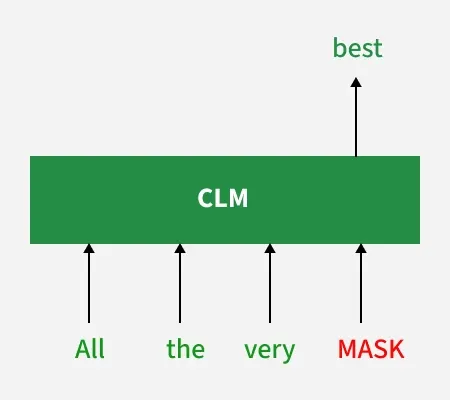
\includegraphics[width=0.8\textwidth]{gpt_clm.png}
    \captionof{figure}{Mục tiêu huấn luyện của GPT: Causal Language Modeling. Tại mỗi bước, mô hình cố gắng dự đoán từ tiếp theo dựa trên các từ trước đó.}
    \label{fig:gpt_clm}
\end{center}

\subsubsection{Sự phát triển và các mô hình tiêu biểu}
Họ mô hình này đã chứng kiến sự phát triển bùng nổ, từ các mô hình tiên phong đến một hệ sinh thái đa dạng các LLMs mã nguồn mở và đóng.

\paragraph{1. Gia đình GPT (OpenAI): Những người tiên phong và dẫn đầu}
Họ mô hình GPT của OpenAI không chỉ định hình nên kiến trúc Decoder-Only mà còn liên tục đẩy lùi các giới hạn của AI.
\begin{itemize}
    \item \textbf{GPT (2018) \cite{radford2018improving}:} Bài báo gốc chứng minh rằng một mô hình Transformer chỉ-Decoder được huấn luyện trước có thể được tinh chỉnh hiệu quả cho các tác vụ NLU.
    \item \textbf{GPT-2 (2019) \cite{radford2019language}:} Gây tiếng vang lớn khi cho thấy việc tăng quy mô (lên tới 1.5 tỷ tham số) có thể tạo ra một mô hình có khả năng sinh văn bản mạch lạc đáng kinh ngạc mà không cần tinh chỉnh (zero-shot).
    \item \textbf{GPT-3 (2020) \cite{brown2020language}:} Mở ra kỷ nguyên LLM thực sự với 175 tỷ tham số. GPT-3 lần đầu tiên thể hiện rõ các \textbf{khả năng nổi trội (emergent abilities)}, đặc biệt là \textbf{học trong ngữ cảnh (in-context learning)}, cho phép nó thực hiện các tác vụ chỉ bằng cách cung cấp vài ví dụ trong prompt (few-shot).
    \item \textbf{InstructGPT \& ChatGPT \cite{ouyang2022training}:} Đánh dấu một bước ngoặt từ "mô hình ngôn ngữ" sang "trợ lý AI" bằng cách sử dụng các kỹ thuật căn chỉnh (alignment) như \textbf{Instruction Tuning} và \textbf{RLHF} (Reinforcement Learning from Human Feedback) để làm cho mô hình hữu ích, trung thực và an toàn hơn.
    \item \textbf{GPT-4 \& GPT-4o (2023-2024) \cite{openai2023gpt4, openai2024gpt4o}:} Là các mô hình SOTA hiện tại, không chỉ mạnh mẽ hơn về ngôn ngữ mà còn trở thành các mô hình \textbf{đa phương thức (multimodal)}, có khả năng hiểu và xử lý cả văn bản, hình ảnh, và âm thanh.
\end{itemize}

\paragraph{2. Làn sóng LLMs Mã nguồn mở và các đối thủ cạnh tranh}
Sự thành công của GPT đã thúc đẩy một làn sóng nghiên cứu và phát triển LLMs trên toàn thế giới, với nhiều mô hình mã nguồn mở mạnh mẽ.
\begin{itemize}
    \item \textbf{LLaMA (Meta) \cite{touvron2023llama}:} Họ mô hình LLaMA (và các phiên bản kế nhiệm LLaMA 2, LLaMA 3) đã "dân chủ hóa" LLMs, cung cấp các mô hình mã nguồn mở có hiệu năng cực kỳ cạnh tranh, tạo điều kiện cho một hệ sinh thái ứng dụng và nghiên cứu khổng lồ.
    \item \textbf{Mistral (Pháp):} Nổi lên như một đối thủ đáng gờm với các mô hình hiệu năng cao nhưng kích thước nhỏ gọn (ví dụ: Mistral 7B \cite{jiang2023mistral}). Họ cũng đi tiên phong trong việc thương mại hóa kiến trúc \textbf{Mixture of Experts (MoE)} với mô hình Mixtral, giúp tăng đáng kể số lượng tham số mà không tăng chi phí suy luận tương ứng.
    \item \textbf{Claude (Anthropic):} Được biết đến với "cửa sổ ngữ cảnh" (context window) rất lớn và tập trung mạnh vào sự an toàn thông qua phương pháp \textbf{Constitutional AI} \cite{bai2022constitutional}.
    \item \textbf{Các mô hình đáng chú ý khác:}
        \begin{itemize}
            \item \textbf{Google:} Gemma (mã nguồn mở), Gemini (mô hình SOTA cạnh tranh với GPT-4).
            \item \textbf{Cohere:} Command R(+), tập trung vào các ứng dụng doanh nghiệp và Retrieval-Augmented Generation (RAG).
            \item \textbf{Các mô hình từ Trung Quốc:} Qwen (Alibaba), Yi, Baichuan, InternLM, DeepSeek, thể hiện sự tiến bộ nhanh chóng của cộng đồng AI Trung Quốc.
            \item \textbf{TII (UAE):} Falcon.
        \end{itemize}
\end{itemize}

\paragraph{3. Các mô hình Decoder-Only chuyên biệt}
Bên cạnh các LLM đa dụng, nhiều mô hình được huấn luyện đặc biệt cho các miền cụ thể.
\begin{itemize}
    \item \textbf{Code LLMs:} Các mô hình được huấn luyện chủ yếu trên dữ liệu mã nguồn để hỗ trợ lập trình. Ví dụ: Codex \cite{chen2021evaluating} (nền tảng của GitHub Copilot đời đầu), StarCoder\cite{li2023starcoder}, CodeLLaMA \cite{roziere2023code}, Phi-3 (Microsoft).
    \item \textbf{Dialogue-focused Models:} Các mô hình được tinh chỉnh đặc biệt cho các tác vụ hội thoại, là tiền thân của các chatbot hiện đại. Ví dụ: DialoGPT (Microsoft) \cite{zhang2019dialogpt}, ChatGLM (Trung Quốc).
\end{itemize}

\begin{tcolorbox}[
    title=Tổng kết: Điểm mạnh và Ứng dụng của Decoder-Only,
    colback=red!5!white, colframe=red!75!black, fonttitle=\bfseries
]
\textbf{Nguyên tắc chung:} Sử dụng mô hình Decoder-Only khi tác vụ của bạn đòi hỏi việc \textbf{sinh ra một chuỗi văn bản mới, mạch lạc, và có tính sáng tạo} dựa trên một ngữ cảnh đầu vào. Chúng là các mô hình \textbf{NLG (Natural Language Generation)} và là nền tảng của AI tạo sinh (Generative AI).

\textbf{Điểm mạnh:}
\begin{itemize}
    \item \textbf{Khả năng sinh văn bản xuất sắc:} Là kiến trúc tốt nhất cho mọi tác vụ NLG.
    \item \textbf{Tính linh hoạt (Zero-shot/Few-shot):} Các mô hình lớn có thể thực hiện nhiều tác vụ chỉ thông qua prompt mà không cần fine-tuning, rất linh hoạt và tiết kiệm chi phí gán nhãn.
\end{itemize}
\textbf{Điểm yếu:}
\begin{itemize}
    \item \textbf{Hiểu ngữ cảnh không sâu bằng Encoder-Only:} Do bản chất một chiều, biểu diễn của một từ không được "nhìn thấy" các từ phía sau. Điều này làm chúng kém tối ưu hơn cho các tác vụ NLU thuần túy so với BERT/RoBERTa.
    \item \textbf{Dễ "ảo giác" (Hallucination):} Có xu hướng bịa đặt thông tin một cách tự tin.
    \item \textbf{Quá trình sinh tuần tự là chậm.}
\end{itemize}

\textbf{Ứng dụng điển hình:}
\begin{itemize}
    \item \textbf{Hệ thống Đối thoại và Trợ lý ảo (Chatbots):} ChatGPT, Claude, Gemini.
    \item \textbf{Sáng tạo nội dung:} Viết văn, làm thơ, soạn email, tóm tắt văn bản (abstractive summarization).
    \item \textbf{Lập trình và Sinh mã (Code Generation):} GitHub Copilot.
    \item \textbf{Giải quyết vấn đề thông qua Prompting:} Bất kỳ tác vụ nào có thể được định dạng dưới dạng "đầu vào -> đầu ra văn bản", từ dịch máy, trả lời câu hỏi, đến lý luận toán học.
\end{itemize}
\end{tcolorbox}


\subsection{Họ Mô hình Encoder-Decoder: Sự kết hợp của hai thế giới}
\label{ssec:encoder_decoder_models}
Họ mô hình này quay trở lại với kiến trúc Transformer gốc ("Attention is All You Need"), sử dụng cả hai thành phần Encoder và Decoder. Mặc dù không còn là tâm điểm chú ý như các LLM Decoder-Only, chúng vẫn là kiến trúc mạnh mẽ và phù hợp nhất cho nhiều tác vụ chuỗi-sang-chuỗi quan trọng.

\begin{tcolorbox}[
    title=Triết lý của Encoder-Decoder,
    colback=green!5!white, colframe=green!60!black, fonttitle=\bfseries
]
"Tôi sẽ dùng một bộ mã hóa hai chiều mạnh mẽ để \textbf{hiểu trọn vẹn} văn bản nguồn, và sau đó dùng một bộ giải mã tự hồi quy để \textbf{sinh ra} văn bản đích dựa trên sự hiểu biết đó."
\end{tcolorbox}

\subsubsection{Kiến trúc và Lợi thế Cốt lõi}
\begin{itemize}
    \item \textbf{Kiến trúc:} Một Encoder hai chiều (giống BERT) để đọc và hiểu toàn bộ chuỗi đầu vào. Một Decoder một chiều (giống GPT) để sinh ra chuỗi đầu ra. Hai thành phần này được kết nối với nhau thông qua cơ chế \textbf{Cross-Attention}, cho phép Decoder "tham khảo" bất kỳ phần nào của chuỗi đầu vào đã được mã hóa ở mỗi bước sinh từ.
    \item \textbf{Lợi thế Cốt lõi:} Sự phân tách vai trò này là một lợi thế không thể thay thế trong các tác vụ đòi hỏi sự hiểu biết sâu sắc về toàn bộ ngữ cảnh nguồn trước khi tạo ra đầu ra. Encoder có thể xây dựng một biểu diễn hai chiều hoàn chỉnh, nắm bắt các mối quan hệ phức tạp trong văn bản nguồn. Decoder sau đó có thể tận dụng biểu diễn phong phú này để tạo ra một đầu ra chính xác và phù hợp hơn.
\end{itemize}

\subsubsection{Sự phát triển và các mô hình tiêu biểu}
Họ Encoder-Decoder có một lịch sử phát triển phong phú, từ mô hình nền tảng đến các biến thể được tối ưu hóa cao cho các tác vụ chuyên biệt.

\paragraph{1. Các mô hình Nền tảng và Đa ngôn ngữ}
\begin{itemize}
    \item \textbf{Transformer (Google, 2017) \cite{vaswani2017attention}:} Bài báo "Attention Is All You Need" chính là khởi nguồn của tất cả. Nó giới thiệu kiến trúc Encoder-Decoder với Self-Attention và đã thay thế hoàn toàn RNN trong các tác vụ dịch máy SOTA thời bấy giờ.
    \item \textbf{T5 (Google, 2019) \cite{raffel2020exploring}:} Phổ biến hóa khung làm việc "Text-to-Text", đối xử mọi bài toán NLP như một tác vụ Seq2Seq, giúp đơn giản hóa và thống nhất quá trình nghiên cứu và ứng dụng.
    \item \textbf{BART (Facebook, 2019) \cite{lewis2019bart}:} Kết hợp các ý tưởng từ BERT (encoder hai chiều) và GPT (decoder tự hồi quy) với mục tiêu huấn luyện khử nhiễu linh hoạt, đặc biệt mạnh mẽ cho các tác vụ sinh văn bản có điều kiện.
    \item \textbf{Các phiên bản Đa ngôn ngữ:} Thành công của các mô hình trên đã dẫn đến các phiên bản đa ngôn ngữ được huấn luyện trên hàng trăm thứ tiếng, bao gồm \textbf{mT5}, \textbf{mBART}, và \textbf{MarianMT} (một mô hình từ Microsoft/Facebook được tối ưu hóa cao cho dịch máy). Gần đây nhất, \textbf{NLLB (No Language Left Behind) \cite{costa2022no}} của Meta đã đẩy giới hạn này đi xa hơn, tập trung vào các ngôn ngữ ít tài nguyên.
\end{itemize}

\paragraph{2. Các biến thể với Mục tiêu Huấn luyện và Kiến trúc Sáng tạo}
Nhiều mô hình đã cải tiến kiến trúc hoặc mục tiêu huấn luyện để đạt hiệu năng vượt trội trên các tác vụ cụ thể, đặc biệt là tóm tắt văn bản.
\begin{itemize}
    \item \textbf{PEGASUS (Google, 2020) \cite{zhang2020pegasus}:} Một mô hình cực kỳ mạnh mẽ cho tóm tắt văn bản. Thay vì che các token (MLM) hay các đoạn (T5), PEGASUS có mục tiêu huấn luyện trước là \textbf{"Gap-Sentences Generation"}. Nó che đi toàn bộ các câu quan trọng trong một tài liệu và yêu cầu mô hình sinh lại các câu đó từ phần còn lại. Điều này mô phỏng rất gần với tác vụ tóm tắt.
    \item \textbf{ProphetNet (Microsoft, 2020) \cite{qi2020prophetnet}:} Cải tiến kiến trúc Decoder để có thể dự đoán \textbf{nhiều bước trong tương lai (future n-gram prediction)} thay vì chỉ một từ tiếp theo. Việc "nhìn xa" này giúp mô hình tránh bị lặp lại và tạo ra các bản tóm tắt chất lượng cao hơn.
    \item \textbf{BERT2BERT \cite{rothe2020leveraging}:} Một kiến trúc đơn giản nhưng hiệu quả, khởi tạo cả Encoder và Decoder bằng các trọng số của một mô hình BERT đã được huấn luyện trước. Đây là một cách "khởi động nóng" (warm-start) hiệu quả cho các tác vụ Seq2Seq như tóm tắt.
    \item \textbf{ByT5 (Google) \cite{xue2022byt5}:} Một biến thể của T5 xử lý trực tiếp \textbf{chuỗi các byte UTF-8} thay vì các token. Cách tiếp cận này loại bỏ sự phức tạp và các lỗi tiềm ẩn của quá trình tokenization, giúp mô hình trở nên mạnh mẽ hơn với nhiễu và đa ngôn ngữ.
\end{itemize}

\paragraph{3. Hướng tới sự Hợp nhất và Linh hoạt}
Các nghiên cứu gần đây tìm cách tạo ra các mô hình linh hoạt hơn, có thể đảm nhận nhiều vai trò khác nhau.
\begin{itemize}
    \item \textbf{UL2 (Google, 2022) \cite{tay2022unifying}:} Giới thiệu một khung làm việc huấn luyện trước \textbf{hợp nhất (unified)}. Bằng cách thay đổi các mục tiêu khử nhiễu, UL2 có thể được huấn luyện để hoạt động như một Encoder-Only, Decoder-Only, hoặc Encoder-Decoder, mở ra hướng đi cho các mô hình đa năng.
    \item \textbf{Flan-T5 (Google):} Là một phiên bản của T5 đã được \textbf{tinh chỉnh theo chỉ dẫn (instruction-tuned) \cite{chung2022scaling}} trên hàng trăm tác vụ NLP được định dạng lại. Quá trình này giúp Flan-T5 có khả năng tổng quát hóa zero-shot đáng kinh ngạc cho các tác vụ mới, một khả năng vốn thường thấy ở các mô hình Decoder-Only. \textbf{Tk-Instruct} cũng là một mô hình tương tự được huấn luyện trên một bộ chỉ dẫn còn lớn hơn.
\end{itemize}

\subsubsection{Khi nào nên sử dụng Họ mô hình Encoder-Decoder?}
\begin{tcolorbox}[
    title=Đánh giá Họ Mô hình Encoder-Decoder,
    colback=green!5!white, colframe=green!60!black, fonttitle=\bfseries
]
\textbf{Nguyên tắc chung:} Sử dụng mô hình Encoder-Decoder khi tác vụ của bạn là một bài toán \textbf{chuỗi-sang-chuỗi (sequence-to-sequence) có điều kiện mạnh mẽ}, nơi chất lượng của đầu ra phụ thuộc rất nhiều vào sự hiểu biết sâu sắc và toàn diện về toàn bộ chuỗi đầu vào.

\textbf{Điểm mạnh:}
\begin{itemize}
    \item \textbf{Hiệu năng SOTA cho các tác vụ Seq2Seq cổ điển:} Là lựa chọn tự nhiên và thường là tốt nhất cho các tác vụ như dịch máy và tóm tắt văn bản, đặc biệt khi cần độ chính xác cao.
    \item \textbf{Kiểm soát tốt hơn:} Việc tách biệt Encoder và Decoder cho phép kiểm soát tốt hơn quá trình mã hóa thông tin nguồn trước khi sinh ra thông tin đích.
\end{itemize}
\textbf{Điểm yếu:}
\begin{itemize}
    \item \textbf{Phức tạp và nhiều tham số hơn:} Phải huấn luyện cả Encoder và Decoder, làm tăng chi phí tính toán và bộ nhớ.
    \item \textbf{Kém linh hoạt trong các tác vụ zero-shot:} So với các mô hình Decoder-Only lớn, chúng thường không có khả năng "học trong ngữ cảnh" (in-context learning) mạnh mẽ và đòi hỏi phải được tinh chỉnh (fine-tuned) cho từng tác vụ cụ thể (ngoại trừ các phiên bản instruction-tuned như Flan-T5).
\end{itemize}
\textbf{Ứng dụng điển hình:}
\begin{itemize}
    \item \textbf{Dịch máy (Machine Translation).}
    \item \textbf{Tóm tắt văn bản (Summarization).}
    \item \textbf{Hỏi-đáp sinh (Generative Question Answering).}
    \item \textbf{Chuyển đổi Dữ liệu-thành-Văn bản (Data-to-text),} ví dụ, sinh mô tả từ một bảng dữ liệu có cấu trúc.
    \item \textbf{Các tác vụ chỉnh sửa văn bản (Text Editing) và tái cấu trúc câu.}
\end{itemize}
\end{tcolorbox}